\problemname{Vasaloppet}
Charlotte tittar på vasaloppet på TV. Sändningen börjar vid tiden $0$ och slutar vid tiden $T$. Tyvärr finns det
också $N$ reklamavbrott, som varar under $N$ icke-överlappande intervall av tid mellan $0$ och $T$. Charlotte blir
väldigt inspirerad av att se de tävlande på startlinjen, och vill därför själv ut och åka skidor under loppet.
Skidturen tar $S$ sekunder, och hon måste vara tillbaka senast vid tiden $T$ (för hon vill se vem som vinner).

Charlotte vill åka på sin skidtur vid ett tillfälle då hon missar så lite av vasaloppet som möjligt. Din uppgift
är att räkna ut det minsta tiden av vasaloppet som Charlotte kan missa om hon optimalt väljer när hon ska åka på sin skidtur.
Missad tid är den tid när Charlotte är ute på sin skidtur samtidigt som det inte är reklampaus.

\begin{centering}
  \begin{figure}[h]
      \centering
      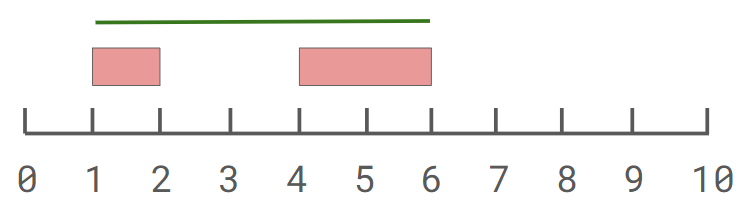
\includegraphics[scale=0.6]{sample1.PNG}
      \caption{Bilden föreställer första exempelfallet. De röda rektanglarna är reklampauserna. Om Charlotte börjar sin skidtur när första pausen börjar och kommer tillbaka när andra pausen slutar så missar hon bara $2$ sekunder av vasaloppet.}
      \label{fig:enter-label}
  \end{figure}
\end{centering}

\section*{Indata}
Den första raden innehåller tre heltal $N,T$ och $S$ ($0 \leq N \leq 10^5$, $1 \leq S \leq T \leq 10^9$).

Därefter följer $N$ rader som vardera innehåller två heltal $l_i, r_i$ ($1 \leq l_i < r_i \leq T$),
vilket betyder att det $i$:te reklamavbrottet varar från och med tid $l_i$ till och med tid $r_i$ (det vill säga inklusive i både $l_i$ och $r_i$).\\
Det gäller dessutom att alla reklamavbrott är disjunkta och sorterade, det vill säga att $r_i < l_{i+1}$ för $i < N$. 

\section*{Utdata}
Skriv ut ett heltal, den minsta tiden av vasaloppet som Charlotte missar under sin skidtur om den väljs optimalt. Notera att skidturen får sluta precis vid tiden $T$. Exempelvis kan skidturen vara under tiderna $1,2,3$ om $S=3, T=3$

\section*{Poängsättning}
Din lösning kommer att testas på en mängd testfallsgrupper.
För att få poäng för en grupp så måste du klara alla testfall i gruppen.

\noindent
\begin{tabular}{| l | l | p{12cm} |}
  \hline
  \textbf{Grupp} & \textbf{Poäng} & \textbf{Gränser} \\ \hline
  $1$    & $10$       & $N=1$ \\ \hline
  $2$    & $25$       & $N \leq 1000$. \\ \hline
  $3$    & $30$       & $T \leq 10^6$. \\ \hline
  $4$    & $35$       & Inga ytterligare begränsningar. \\ \hline
\end{tabular}